\documentclass[10pt, compress]{beamer}

\usetheme[usetitleprogressbar]{m}

\usepackage{booktabs}
\usepackage[scale=2]{ccicons}
\usepackage{minted}
\usepackage{pgfplots}
\usepackage{graphicx, float}
\usepackage{caption}
\usepackage{subcaption}
\usepackage{textpos}
\usepackage{fontawesome}


\newcommand<>{\fullsizegraphic}[1]{
  \begin{textblock*}{0cm}(-1cm,-3.78cm)
  \includegraphics[width=\paperwidth]{#1}
  \end{textblock*}
}



\graphicspath{{./images/}}

%\usepgfplotslibrary{dateplot}

\usepackage{amsthm}
\newtheorem{mydef}{\alert{Definition:}}
\newtheorem{ex}{\alert{Example:}}

\usemintedstyle{trac}

\title{\huge The Beautiful Geometry of Aperiodic Tessellations}
\subtitle{}
\date{\today}
\author{Jesse Bettencourt}
\institute{Supervised by Miroslav Lovric}

\begin{document}

\maketitle
\section{What is a Tessellation?}

\begin{frame}{Figures}
  \frametitle{A Simple Tessellation}
  
  \begin{figure}
	\includegraphics[width=0.5\textwidth]{Checkerboard}
    \caption*{Checkerboard Tessellation}
    \label{fig:checkerboard}
  \end{figure}
  
  
\end{frame}

\begin{frame}[fragile]
  \frametitle{What is a Tessellation?}
\begin{mydef}
A \textbf{tessellation} $\mathcal{T}$ of the space $\mathbb{E}^n$ is a countable family of closed sets, $T$, called \emph{tiles}:
\begin{equation*}
\mathcal{T}=\{T_1,T_2,\mathellipsis\}
\end{equation*}
such that
\begin{enumerate}
\item $\mathcal{T}$ has \textbf{no overlaps}: $\mathring{T_i} \cap \mathring{T_j}=\emptyset$ if $i\neq j$
\item $\mathcal{T}$ has \textbf{no gaps}: $\bigcup_{i=1}^\infty T_i = \mathbb{E}^n$
\end{enumerate}
\end{mydef}

\begin{center}
\includegraphics[width=0.2\textwidth]{Checkerboard}
\end{center}
\end{frame}



\begin{frame}[fragile]
\frametitle{Components of a Tessellation}

\begin{mydef}
Let $\{T_1,T_2,\mathellipsis\}$ be the set of tiles of tessellation $\mathcal{T}$, partitioned into a set of equivalence classes by \textbf{criterion} $\mathcal{M}$. The set, $\mathcal{P}$, of representatives of these equivalence classes is called the \textbf{protoset} for $\mathcal{T}$ with respect to $\mathcal{M}$.
\end{mydef}

\begin{ex}
\begin{table}
\begin{tabular}{l c}
  \textbf{Criterion:} & $\mathcal{M}=$ \{\emph{Colour of the tile. Only opposite colours may touch.}\}\\[10pt]
  \textbf{Protoset:} &  
     \huge  \raisebox{0pt}{$\mathcal{P}=$ \{} 
                  \raisebox{-10pt}{
\includegraphics[width=0.1\textwidth]{tealproto}}\raisebox{0pt}{ ,}
                   \raisebox{-10pt}{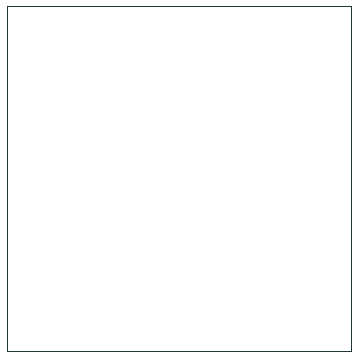
\includegraphics[width=0.1\textwidth]{whiteproto}}
          \huge\raisebox{0pt}{\}}\\
\end{tabular}
\end{table}
\end{ex}

\end{frame}


\begin{frame}[fragile]
\frametitle{Protosets Admit Tessellations}
\begin{mydef}
If $\mathcal{T}$ is a tessellation with protoset $\mathcal{P}$, then we say that $\mathcal{P}$ admits $\mathcal{T}$.
\end{mydef}


\begin{ex}
\flushleft We say\\
\centering\huge \raisebox{0pt}{$\mathcal{P}=$ \{} 
                  \raisebox{0pt}{
\includegraphics[width=0.05\textwidth]{tealproto}}\raisebox{0pt}{ ,}
                   \raisebox{0pt}{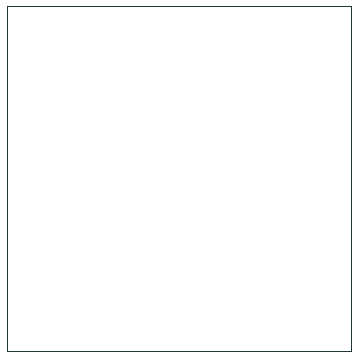
\includegraphics[width=0.05\textwidth]{whiteproto}}
          \huge\raisebox{0pt}{\}}\\
\flushleft\normalsize \raisebox{15pt}{admits}\\
\centering\includegraphics[width=0.2\textwidth]{Checkerboard}
\end{ex}
\end{frame}

\begin{frame}{Figures}
\frametitle{Protosets Can Admit Multiple Tessellations}
\centering\huge \raisebox{0pt}{$\mathcal{P}=$ \{} 
                  \raisebox{0pt}{
\includegraphics[width=0.05\textwidth]{tealproto}}\raisebox{0pt}{ ,}
                   \raisebox{0pt}{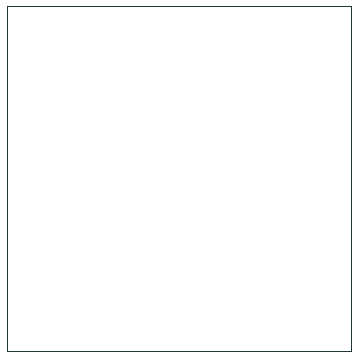
\includegraphics[width=0.05\textwidth]{whiteproto}}
          \huge\raisebox{0pt}{\}}\\
\flushleft\normalsize \raisebox{15pt}{admits both}\\

\begin{figure}
\begin{subfigure}[b]{0.4\textwidth}
\includegraphics[width=\textwidth]{Checkerboard}
\end{subfigure}\hfill \raisebox{60pt}{and} \hfill
\begin{subfigure}[b]{0.4\textwidth}
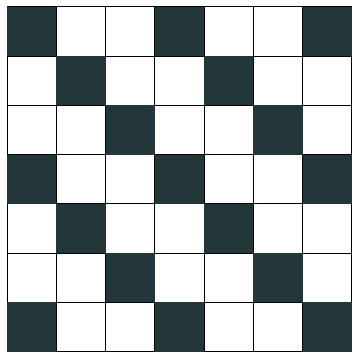
\includegraphics[width=\textwidth]{CheckerboardOther}
\end{subfigure}
\end{figure}
\end{frame}

\begin{frame}{Figures}
\frametitle{Matching Rules Correspond to Deformed Protosets}
\centering
Edge deformations can force matching rules.

\centering\huge \raisebox{0pt}{$\mathcal{P}=$ \{} 
                  \raisebox{0pt}{
\includegraphics[width=0.05\textwidth]{tealproto}}\raisebox{0pt}{ ,}
                   \raisebox{0pt}{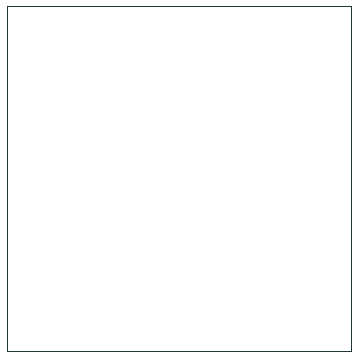
\includegraphics[width=0.05\textwidth]{whiteproto}}
          \huge\raisebox{0pt}{\}}\hfill
          \huge \raisebox{0pt}{$\mathcal{P}=$ \{} 
                            \raisebox{0pt}{
\includegraphics[width=0.05\textwidth]{protodisk}}\raisebox{0pt}{ ,}
                             \raisebox{0pt}{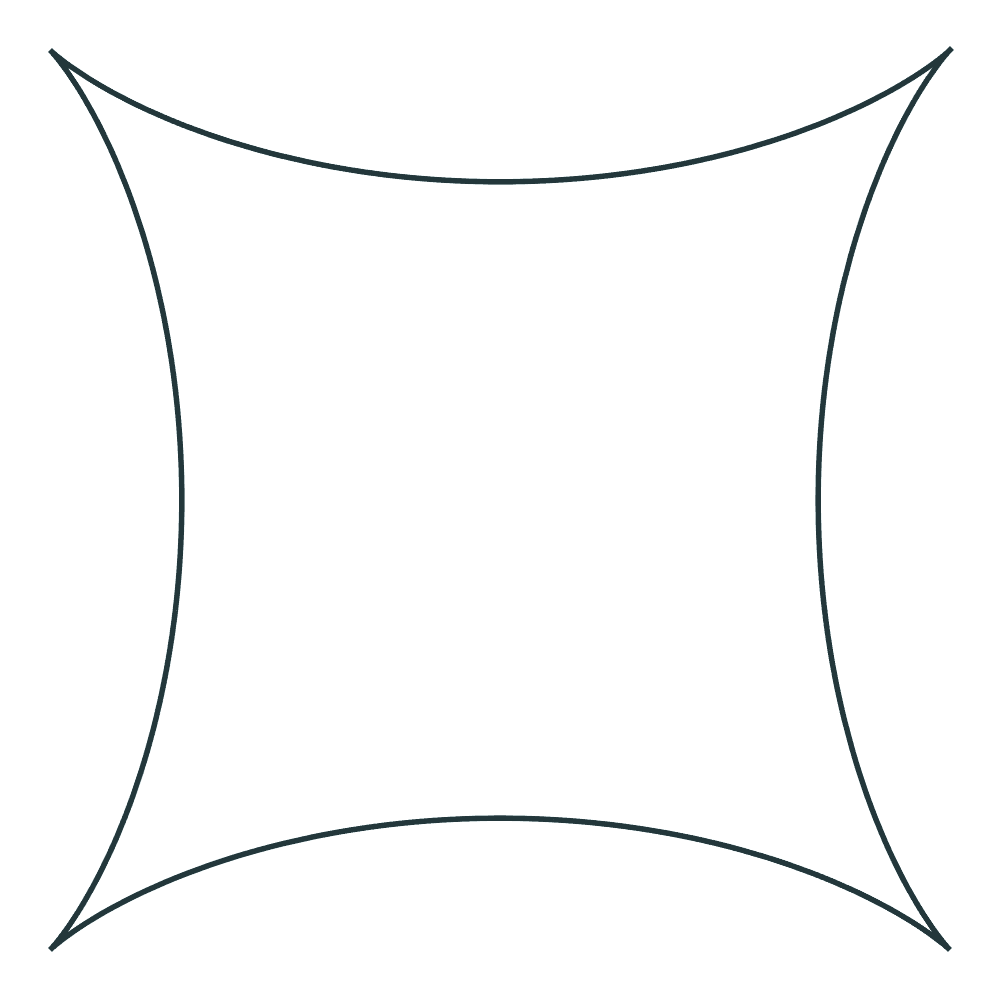
\includegraphics[width=0.05\textwidth]{protosquare}}
                    \huge\raisebox{0pt}{\}}\\
\begin{figure}
\begin{subfigure}[b]{0.3\textwidth}
\includegraphics[width=\textwidth]{Checkerboard}
\end{subfigure}\hfill \raisebox{40pt}{$\rightarrow$} \hfill
\begin{subfigure}[b]{0.3\textwidth}
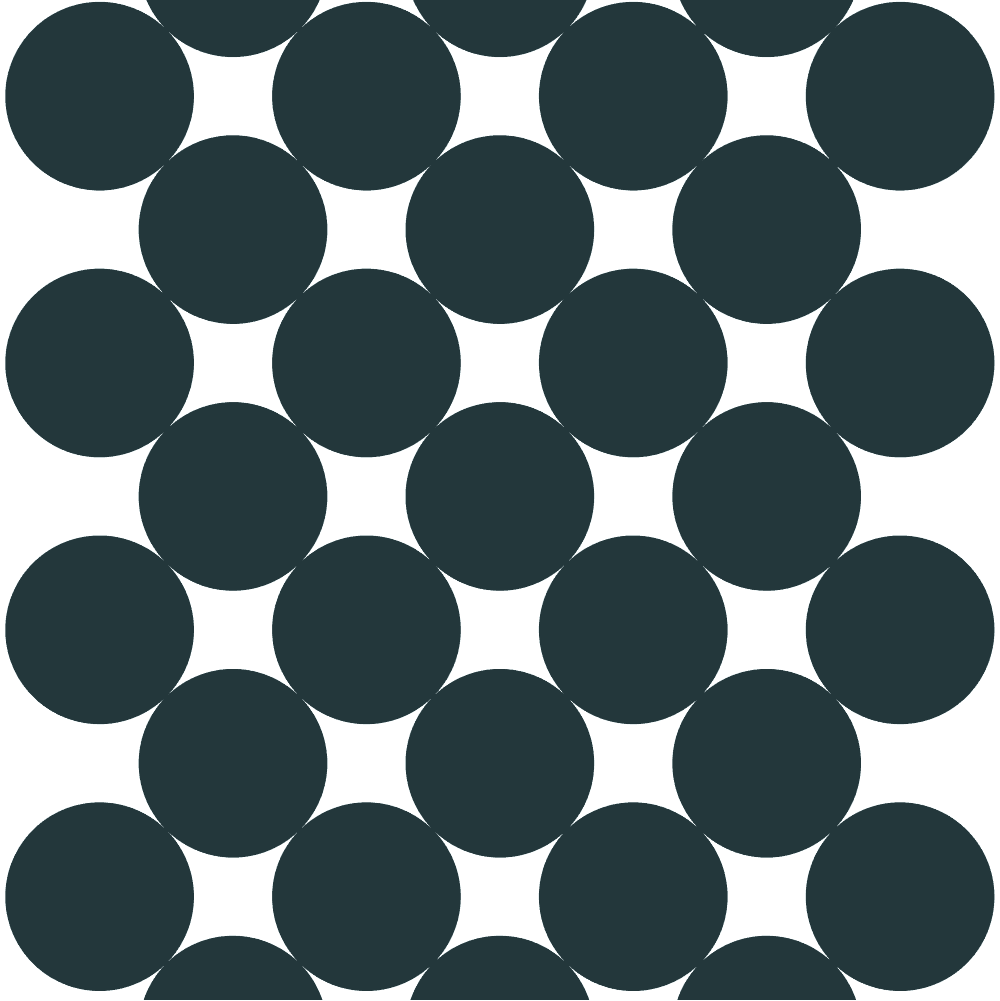
\includegraphics[width=\textwidth]{CheckerboardCircles}
\end{subfigure}
\end{figure}

\normalsize Matching Rules $\implies$ Deformed Protoset
\end{frame}

\section{Describing Tessellations}

%\begin{frame}
%\frametitle{Symmetries}
%
%\begin{mydef}
%A tessellation is said to be \textbf{symmetric} under a transformation if that transformation maps the tiling to itself identically.
%\end{mydef}
%
%\alert{Rotational Symmetry:} $\mathcal{T}$ can be rotated a non-trivial angle about a point and overlap itself identically\\[10pt]
%\alert{Translational Symmetry:} $\mathcal{T}$ can be shifted by some non-trivial distance in a direction and overlap itself identically.
%\end{frame}
%
%\begin{frame}{Figures}
%\frametitle{Checkerboard Symmetries}
%\begin{figure}
%\begin{subfigure}[b]{0.45\textwidth}
%\includegraphics[width=\textwidth]{Checkerboard}
%\caption*{Translation Symmetry: 2 Squares\\ Rotational Symmetry: $\frac{\pi}{2}$}
%\end{subfigure}\hfill
%\begin{subfigure}[b]{0.45\textwidth}
%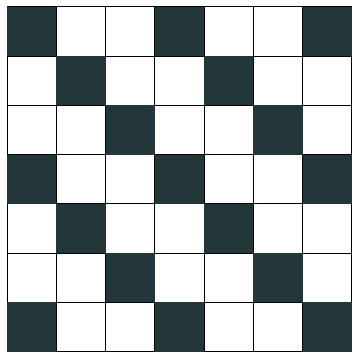
\includegraphics[width=\textwidth]{CheckerboardOther}
%\caption*{Translation Symmetry: 3 Squares\\ Rotational Symmetry: $\pi$}
%\end{subfigure}
%\end{figure}
%\end{frame}

\begin{frame}
\frametitle{Periodicity}
\begin{mydef}
A tessellation is said to be \textbf{periodic} if it admits translational symmetry in two directions.
\end{mydef}
\begin{mydef}
A tessellation is said to be \textbf{non-periodic} if it admits no translational symmetries.
\end{mydef}

\begin{figure}
\begin{subfigure}[b]{0.25\textwidth}
\includegraphics[width=\textwidth]{Checkerboard}
\caption*{Periodic}
\end{subfigure}\hfill
\begin{subfigure}[b]{0.25\textwidth}
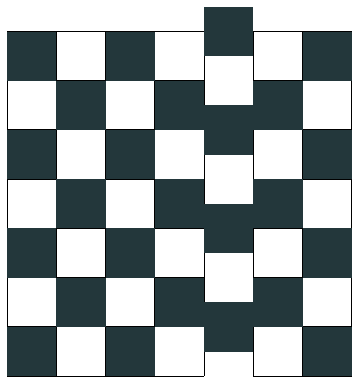
\includegraphics[width=\textwidth]{CheckerboardAperiodic}
\caption*{Non-Periodic}
\end{subfigure}
\end{figure}

\end{frame}



\begin{frame}
\frametitle{The Aperiodic Question}

\centering
Checkerboard protoset,\\
\huge \raisebox{0pt}{$\mathcal{P}=$ \{} 
                  \raisebox{0pt}{
\includegraphics[width=0.05\textwidth]{tealproto}}\raisebox{0pt}{ ,}
                   \raisebox{0pt}{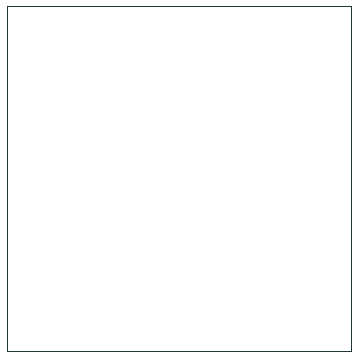
\includegraphics[width=0.05\textwidth]{whiteproto}}
          \huge\raisebox{0pt}{\}}\\ \normalsize admits \alert{both} \textbf{periodic} and \textbf{non-periodic} tessellations.\\[15pt]


\begin{figure}
\begin{subfigure}[b]{0.35\textwidth}
\includegraphics[width=\textwidth]{Checkerboard}
\caption*{Periodic}
\end{subfigure}\hfill
\begin{subfigure}[b]{0.35\textwidth}
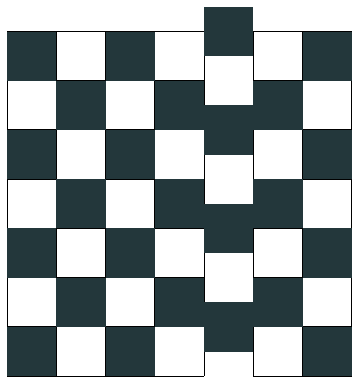
\includegraphics[width=\textwidth]{CheckerboardAperiodic}
\caption*{Non-Periodic}
\end{subfigure}
\end{figure}

\end{frame}

\begin{frame}
\frametitle{The Aperiodic Question}

\centering
Checkerboard protoset,\\
\huge \raisebox{0pt}{$\mathcal{P}=$ \{} 
                  \raisebox{0pt}{
\includegraphics[width=0.05\textwidth]{tealproto}}\raisebox{0pt}{ ,}
                   \raisebox{0pt}{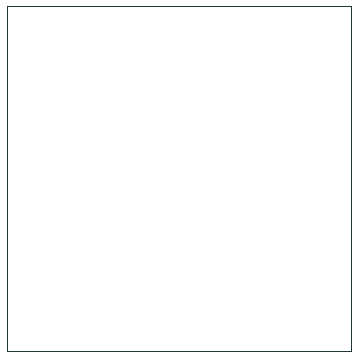
\includegraphics[width=0.05\textwidth]{whiteproto}}
          \huge\raisebox{0pt}{\}}\\ \normalsize admits \alert{both} \textbf{periodic} and \textbf{non-periodic} tessellations.\\[15pt]

Some protosets,\\
\huge \raisebox{0pt}{$\mathcal{P}=$ \{} 
                            \raisebox{0pt}{
\includegraphics[width=0.05\textwidth]{protodisk}}\raisebox{0pt}{ ,}
                             \raisebox{0pt}{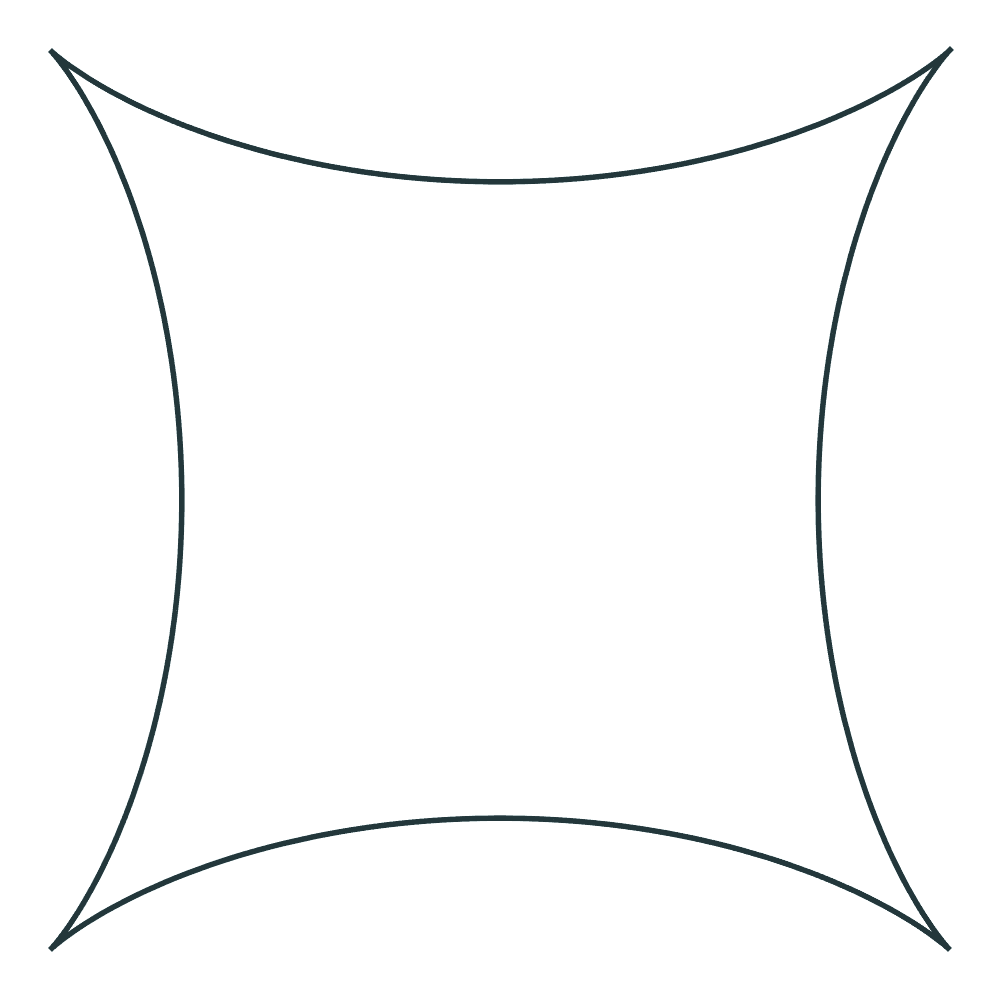
\includegraphics[width=0.05\textwidth]{protosquare}}
                    \huge\raisebox{0pt}{\}}\\ \normalsize admit \alert{only} \textbf{periodic} tessellations.\\[15pt]

\begin{figure}
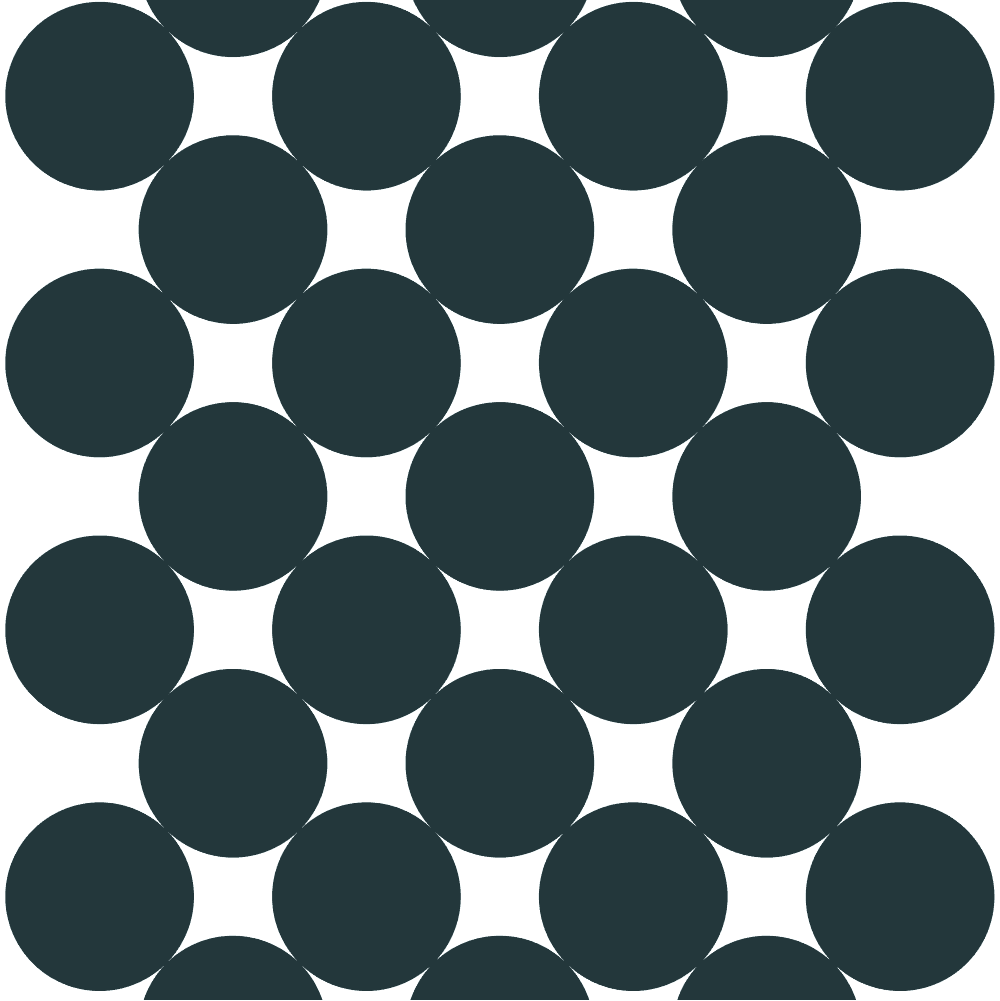
\includegraphics[width=0.2\textwidth]{CheckerboardCircles}
\end{figure}

\invisible{
\begin{figure}
\begin{subfigure}[b]{0.35\textwidth}
\includegraphics[width=\textwidth]{Checkerboard}
\caption*{Periodic}
\end{subfigure}\hfill
\begin{subfigure}[b]{0.35\textwidth}
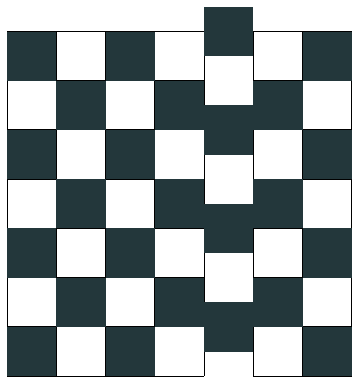
\includegraphics[width=\textwidth]{CheckerboardAperiodic}
\caption*{Non-Periodic}
\end{subfigure}
\end{figure}
}
\end{frame}

\begin{frame}
\frametitle{The Aperiodic Question}

\centering
Checkerboard protoset,\\
\huge \raisebox{0pt}{$\mathcal{P}=$ \{} 
                  \raisebox{0pt}{
\includegraphics[width=0.05\textwidth]{tealproto}}\raisebox{0pt}{ ,}
                   \raisebox{0pt}{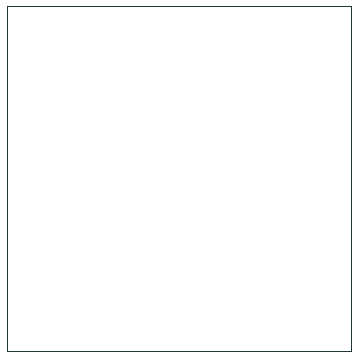
\includegraphics[width=0.05\textwidth]{whiteproto}}
          \huge\raisebox{0pt}{\}}\\ \normalsize admits \alert{both} \textbf{periodic} and \textbf{non-periodic} tessellations.\\[15pt]

Some protosets,\\
\huge \raisebox{0pt}{$\mathcal{P}=$ \{} 
                            \raisebox{0pt}{
\includegraphics[width=0.05\textwidth]{protodisk}}\raisebox{0pt}{ ,}
                             \raisebox{0pt}{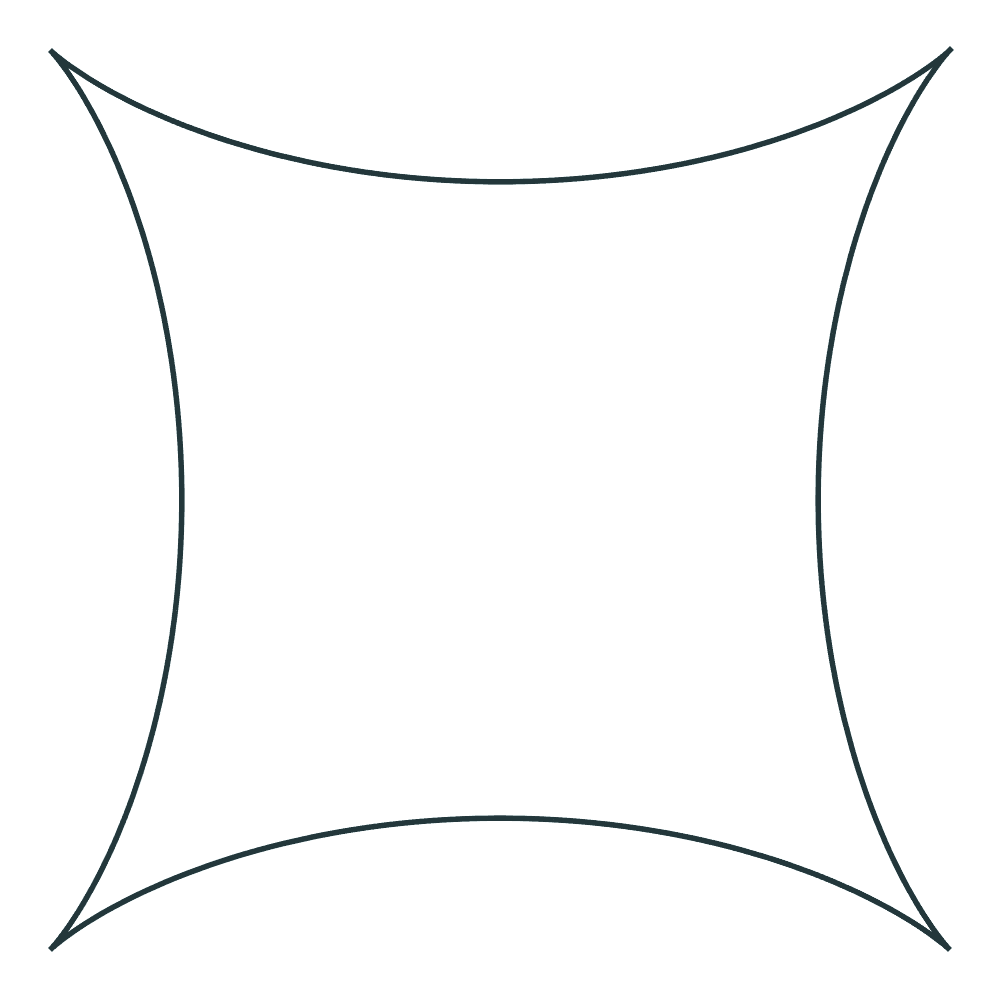
\includegraphics[width=0.05\textwidth]{protosquare}}
                    \huge\raisebox{0pt}{\}}\\ \normalsize admit \alert{only} \textbf{periodic} tessellations.\\[15pt]
          
Are there any protosets,\\
\huge \raisebox{0pt}{$\mathcal{P}=$ \{?\}}\\ 
\normalsize that admit \alert{only} \textbf{non-periodic} tessellations?
\invisible{
\begin{figure}
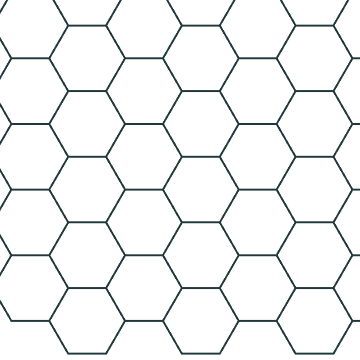
\includegraphics[width=0.2\textwidth]{Hexagons}
\end{figure}
}

\invisible{
\begin{figure}
\begin{subfigure}[b]{0.35\textwidth}
\includegraphics[width=\textwidth]{Checkerboard}
\caption*{Periodic}
\end{subfigure}\hfill
\begin{subfigure}[b]{0.35\textwidth}
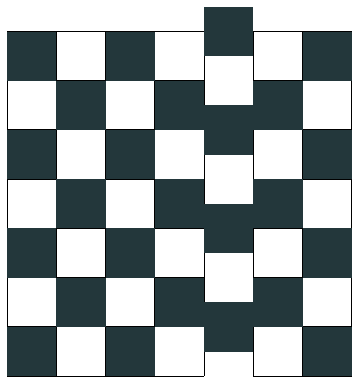
\includegraphics[width=\textwidth]{CheckerboardAperiodic}
\caption*{Non-Periodic}
\end{subfigure}
\end{figure}
}


\begin{figure}
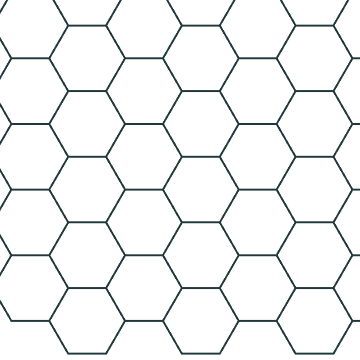
\includegraphics[width=0.2\textwidth]{Hexagons}
\end{figure}

\invisible{
\begin{figure}
\begin{subfigure}[b]{0.35\textwidth}
\includegraphics[width=\textwidth]{Checkerboard}
\caption*{Periodic}
\end{subfigure}\hfill
\begin{subfigure}[b]{0.35\textwidth}
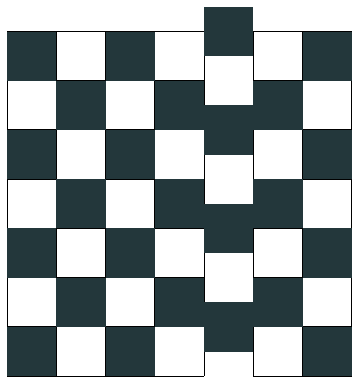
\includegraphics[width=\textwidth]{CheckerboardAperiodic}
\caption*{Non-Periodic}
\end{subfigure}
\end{figure}
}
\end{frame}



\section{An Aperiodic Tessellation}

\begin{frame}
\frametitle{The Penrose Rhombs Protoset}
\centering
\huge \raisebox{25pt}{$\mathcal{P}=$ \{} 
                  \raisebox{0pt}{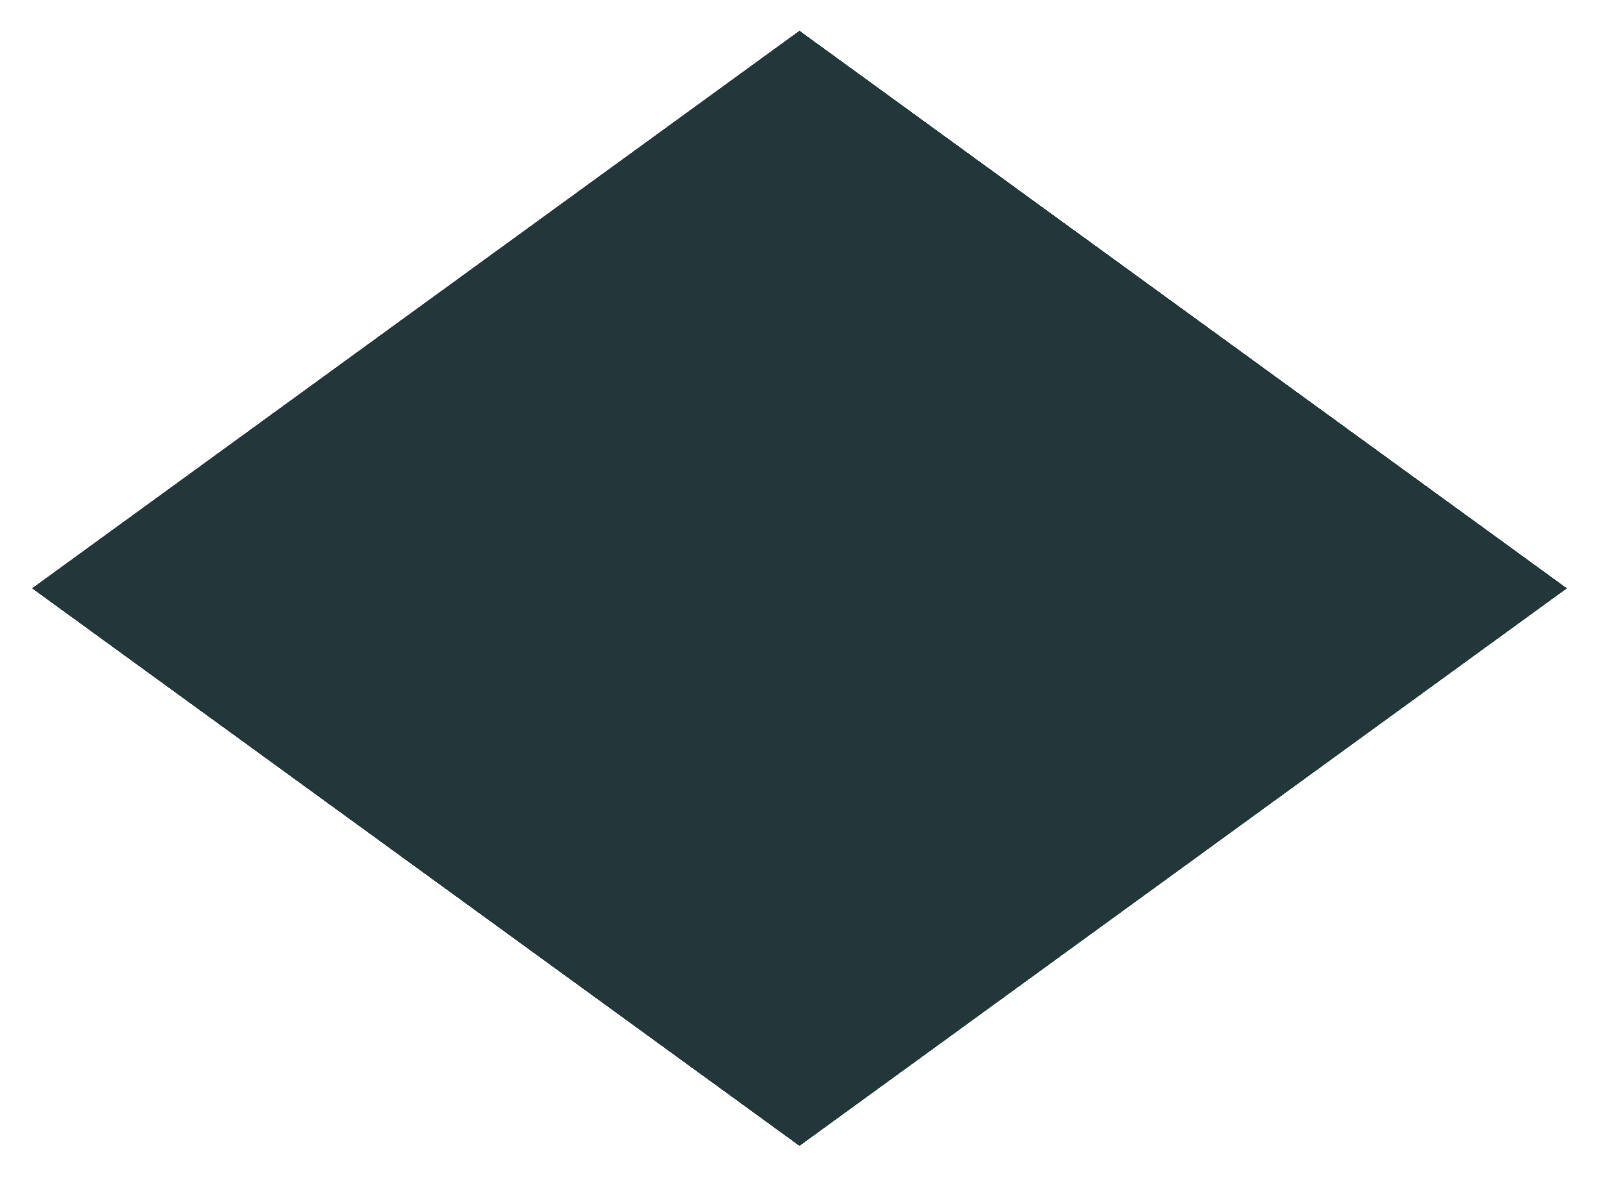
\includegraphics[width=0.3\textwidth]{FatProto}}\raisebox{20pt}{ ,}
                   \raisebox{-10pt}{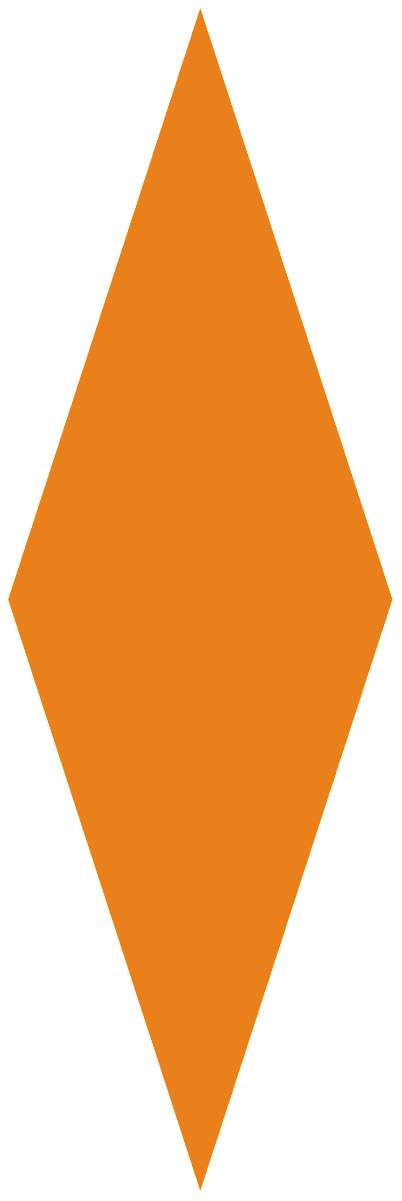
\includegraphics[width=0.1\textwidth]{SkinnyProto}}
          \huge\raisebox{25pt}{\}*}
          
\vfill \raisebox{-7pt}{*} \normalsize With matching rules
\end{frame}

\begin{frame}
\frametitle{The Penrose Rhombs Protoset}
\centering
\huge \raisebox{25pt}{$\mathcal{P}=$ \{} 
                  \raisebox{0pt}{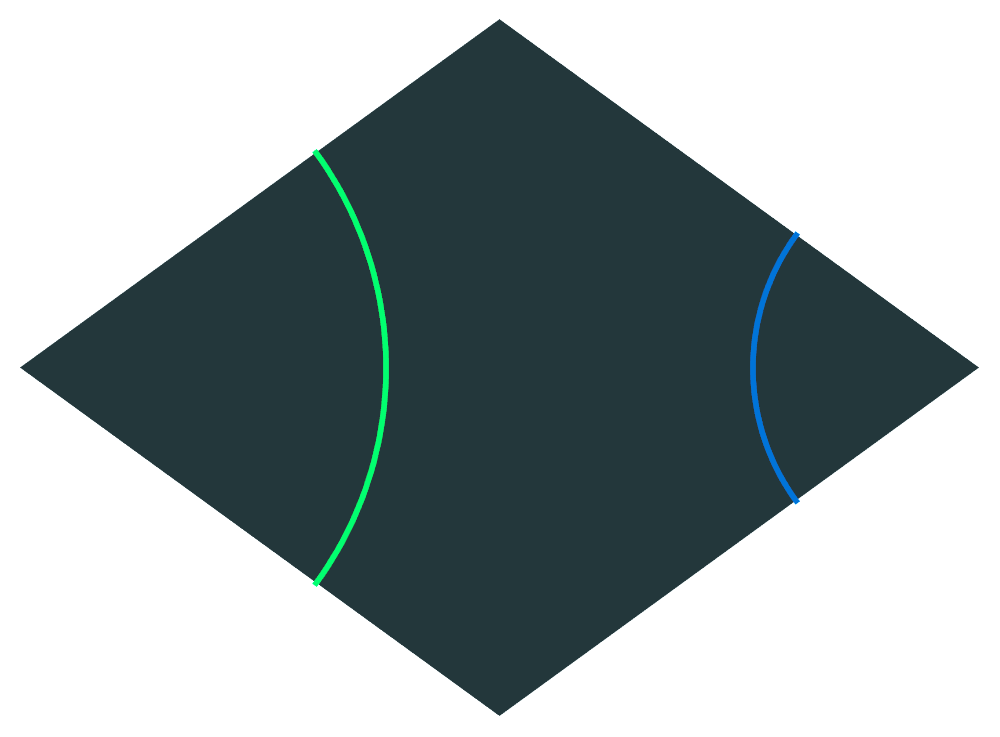
\includegraphics[width=0.3\textwidth]{FatProtoRules}}\raisebox{20pt}{ ,}
                   \raisebox{-10pt}{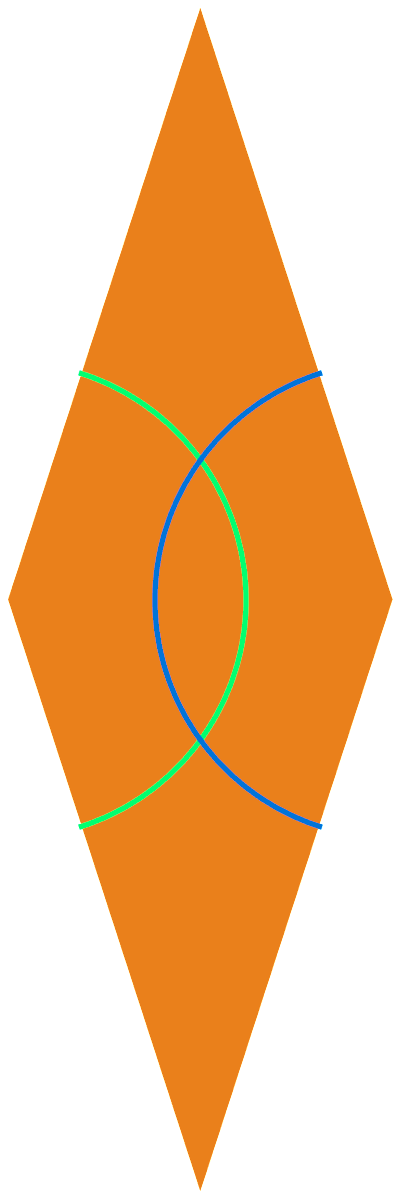
\includegraphics[width=0.1\textwidth]{SkinnyProtoRules}}
          \huge\raisebox{25pt}{\}}
          
\normalsize admits \alert{only} \textbf{non-periodic} tessellations, called Penrose Tessellations.
\end{frame}


\begin{frame}
\frametitle{Non-Locality of the Penrose Tessellations}
Cannot be constructed through \alert{local} procedures.

\begin{ex}
This arrangement

\begin{figure}
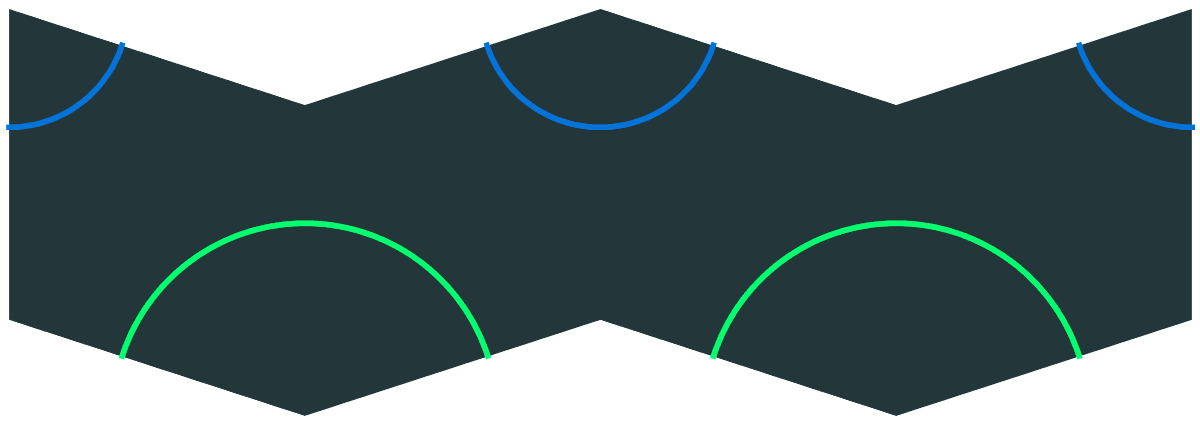
\includegraphics[width=0.6\textwidth]{Mistake}
\end{figure}

follows the matching rules.
\end{ex}
\end{frame}

\begin{frame}
\frametitle{Non-Locality of the Penrose Tessellations}
Cannot be constructed through \alert{local} procedures.
\begin{ex}
This arrangement

\begin{figure}
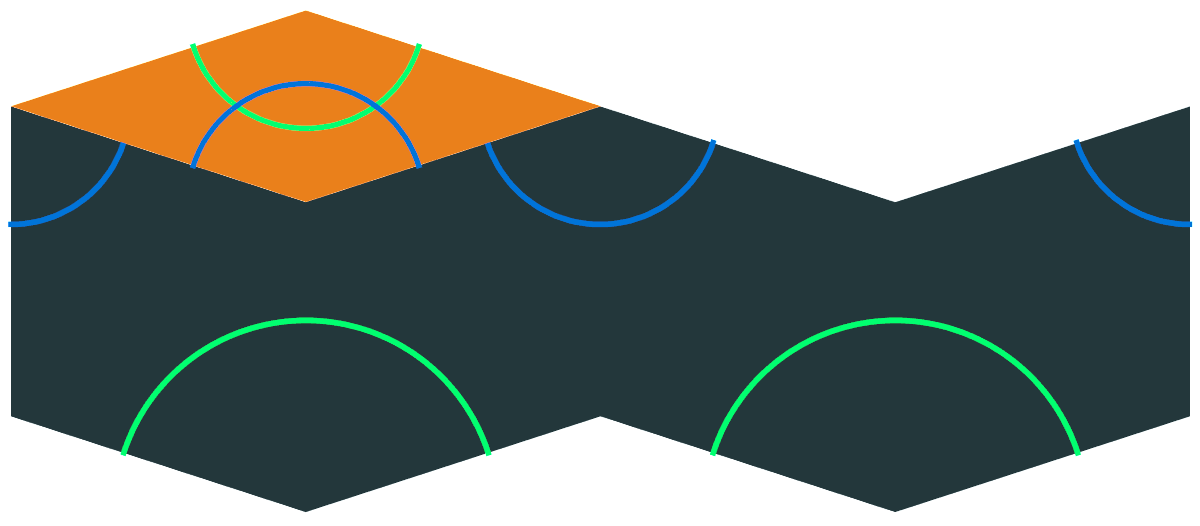
\includegraphics[width=0.6\textwidth]{MistakeNext}
\end{figure}

follows the matching rules, but is a \alert{mistake}!
\end{ex}
\end{frame}


\section{Construction by Substitution}




\begin{frame}
\frametitle{Substitution Rules on Robinson Triangles}
First, consider the Rhombs as joined triangles:

\begin{table}
\begin{tabular}{cccr}
\raisebox{18pt}{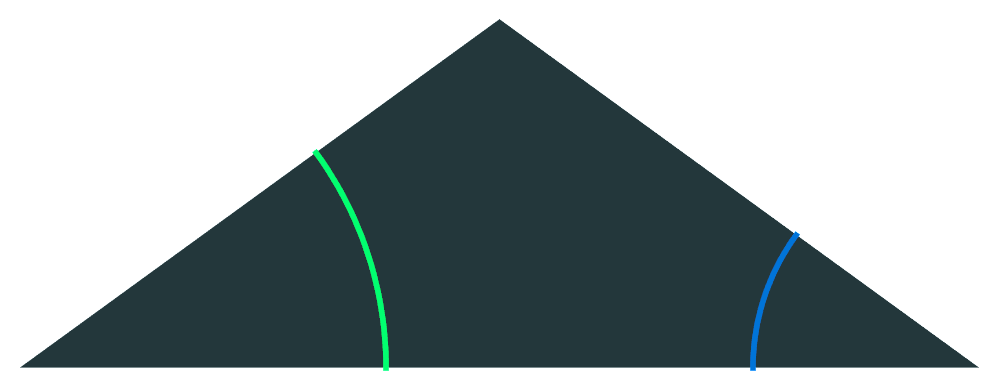
\includegraphics[width=0.4\textwidth]{FatRob}} &
 \huge\raisebox{30pt}{$\rightarrow$} &
\raisebox{10pt}{\includegraphics[width=0.4\textwidth]{RobFatSub}} & \\
\raisebox{10pt}{\includegraphics[width=0.2\textwidth]{SkinnyRob}} &
 \huge\raisebox{30pt}{$\rightarrow$} &
\raisebox{10pt}{\includegraphics[width=0.2\textwidth]{RobSkinnySub}} & \\
\end{tabular}
\end{table}

\end{frame}

\begin{frame}
\frametitle{Substitution Rules on Penrose Rhombs}


\begin{table}
\begin{tabular}{cccr}
\raisebox{25pt}{\includegraphics[width=0.25\textwidth]{FatRhomb}} &
 \huge\raisebox{50pt}{$\rightarrow$} &
\raisebox{10pt}{\includegraphics[width=0.25\textwidth]{RhombFatSubEdge}} & \\
\raisebox{20pt}{\includegraphics[width=0.1\textwidth]{SkinnyRhomb}} &
 \huge\raisebox{60pt}{$\rightarrow$} &
\raisebox{10pt}{\includegraphics[width=0.25\textwidth]{RhombSkinnySubEdge}} & \\
\end{tabular}
\end{table}

\end{frame}

\begin{frame}
\frametitle{Substitution Rules on Penrose Rhombs}


\begin{table}
\begin{tabular}{cccr}
\raisebox{25pt}{\includegraphics[width=0.25\textwidth]{FatRhomb}} &
 \huge\raisebox{50pt}{$\rightarrow$} &
\raisebox{10pt}{\includegraphics[width=0.25\textwidth]{RhombFatSub}} & \\
\raisebox{20pt}{\includegraphics[width=0.1\textwidth]{SkinnyRhomb}} &
 \huge\raisebox{60pt}{$\rightarrow$} &
\raisebox{10pt}{\includegraphics[width=0.25\textwidth]{RhombSkinnySub}} & \\
\end{tabular}
\end{table}

\end{frame}


\begin{frame}
\frametitle{Start with a Seed: Thick Rhombus}
\begin{figure}
\includegraphics[width=0.6\textwidth]{Inflate0}
\end{figure}

\end{frame}

\begin{frame}
\frametitle{Apply Substitution Rules}
\begin{figure}
\includegraphics[width=0.6\textwidth]{Inflate1}
\end{figure}

\end{frame}

\begin{frame}
\frametitle{Apply Substitution Rules Again}
\begin{figure}
\includegraphics[width=0.6\textwidth]{Inflate2}
\end{figure}

\end{frame}

\begin{frame}
\frametitle{Apply Substitution Rules Again and Again}
\begin{figure}
\includegraphics[width=0.6\textwidth]{Inflate3}
\end{figure}

\end{frame}

\begin{frame}
\frametitle{Apply Substitution Rules Again and Again and Again}
\begin{figure}
\includegraphics[width=0.6\textwidth]{Inflate4}
\end{figure}

\end{frame}

\begin{frame}
\frametitle{Apply Substitution Rules Again and Again and Again and Again}
\begin{figure}
\includegraphics[width=0.6\textwidth]{Inflate5}
\end{figure}

\end{frame}

\begin{frame}
\frametitle{Apply Substitution Rules 10 times}
\begin{figure}
\includegraphics[width=0.9\textwidth]{Inflate10}
\end{figure}

\end{frame}

\begin{frame}
\frametitle{Apply Substitution Rules 11 times}

  \fullsizegraphic{Inflate11}
  
\end{frame}




\section{Penrose Tessellation Features}

\begin{frame}
\frametitle{Density of Patterns}
\centering
\large
Any pattern with diameter \alert{$d$} will begin repeating within \alert{$2\phi d$} from the perimeter.
  
\end{frame}

\begin{frame}
\frametitle{Density of Patterns}

  \fullsizegraphic{PatternFind1}
  
\end{frame}

\begin{frame}
\frametitle{Density of Patterns}

  \fullsizegraphic{PatternFind2}
  
\end{frame}

\begin{frame}
\frametitle{Density of Patterns}

  \fullsizegraphic{PatternFind3}
  
\end{frame}

\begin{frame}
\frametitle{Density of Patterns}

  \fullsizegraphic{PatternFind5}
  
\end{frame}

\begin{frame}
\frametitle{Surprising Rotational Symmetry}
\centering
\large
Penrose Tessellations can admit \alert{five-fold} rotational symmetry. 


(Impossible for periodic tessellations)
  
\end{frame}

\begin{frame}
\frametitle{Ratio of Thick to Thin Rhombs}
\centering
$\frac{\raisebox{25pt}{\text{\# of }}\raisebox{0pt}{\includegraphics[width=0.25\textwidth]{FatRhomb}}}{\raisebox{70pt}{\text{\# of }}\raisebox{25pt}{\includegraphics[width=0.1\textwidth]{SkinnyRhomb}}}=$ \huge $\phi$

  
\end{frame}

\begin{frame}
\frametitle{Conclusion}
\centering
\Large
Questions?

\vfill
\faGithub \space \space \space \small \url{github.com/jessebett/PenroseTilingThesis}
\end{frame}

\begin{frame}
\frametitle{Bibliography}
\nocite{Conway1986,DeBruijn1981,DeBruijn1990,Gardner1997,Ogawa1999,Penrose1979,Senechal1996}
\tiny

\setbeamertemplate{bibliography item}{\normalsize \faBook}
\bibliographystyle{plain}
\bibliography{bibliography}
\end{frame}
\end{document}
